\documentclass[11pt]{article}

% Using the final ACL style (generates a 2-column, camera-ready format)
\usepackage{acl}

% Standard package includes
\usepackage{times}
\usepackage{latexsym}

% For proper rendering and hyphenation of words containing Latin characters
\usepackage[T1]{fontenc}
% This assumes your files are encoded as UTF8
\usepackage[utf8]{inputenc}

% Improves the layout of the manuscript
\usepackage{microtype}

%Images
\usepackage{graphicx}

% Improves aesthetics of text in the typewriter font
\usepackage{inconsolata}

\title{Pay Predictor: Predicting Median Salary from Skills Listed on Linkedin Job Postings}

% Author formatting adjusted for ACL style
\author{Khang Pham \and Himnish Chhabra \\
  % You can add your university or emails here if needed:
  % University Name \\
  % \texttt{\{email1, email2\}@domain.edu}
}

\begin{document}

\maketitle

\section*{1. Group Members}

Our group consists of two members: Khang Pham and Himnish Chhabra.

Khang will focus on exploratory data analysis, data cleaning, statistical testing, and visual interpretation of results. This includes examining salary distributions, analyzing differences across industries and company sizes, and conducting hypothesis testing such as ANOVA and ANCOVA. Khang will also be responsible for presenting findings through clear visualizations and evaluating overall model performance.

Himnish will be responsible for implementing the predictive modeling pipeline. This includes preparing structured and textual features, building baseline and advanced machine learning models, and tuning model parameters. He will experiment with models such as linear regression, Support Vector Machines (SVMs), and neural networks.

Both members will collaborate on refining features, interpreting results, and writing the final report to ensure the project is cohesive and well-structured.

\section*{2. Motivation}

The goal of this project is to investigate how job descriptions and required skills relate to salary levels in LinkedIn job postings. Specifically, we want to determine whether the textual content of a job posting can be used to predict its listed compensation.

Many job postings either provide wide salary ranges or omit salary information entirely. As research on pay transparency suggests \cite{arnold2025}, salary information remains inconsistent in online job markets. At the same time, companies compete for talent in an increasingly skill-driven economy. This raises an important question:

\begin{center}
\textit{Can we measure the market value of professional skills directly from job posting data?}
\end{center}

By analyzing job descriptions, industries, and company characteristics, we aim to identify which factors are most strongly associated with higher salaries. Our objective is to better understand how job requirements translate into compensation in today's labor market.

\section*{3. Literature Review}

We will examine prior research on wage determination and salary prediction using online job postings. Previous studies have shown that specific keywords, required skills, and industry trends influence salary outcomes.

In particular, Chen and Autor \cite{chen2024} demonstrate that machine learning models can predict salary levels using textual features from job postings. Their work highlights the importance of language in understanding labor market value.

We will build on this literature by combining statistical hypothesis testing with predictive modeling to evaluate both group-level salary differences and individual salary predictions.

\section*{4. Data}

We will use the LinkedIn Job Postings dataset (2023--2024) available on Kaggle. The dataset contains over 120,000 job listings and includes both structured and unstructured data. Structured variables include job title, company size, industry, location, minimum salary, maximum salary, and pay period. The dataset also includes unstructured text such as job descriptions and listed skills.

Before analysis, we will clean the dataset by removing extreme or unrealistic salary outliers and handling missing salary values. Because the dataset is relatively large, we may apply sampling techniques during model training to improve computational efficiency while maintaining representative results.

\begin{figure}
    \centering
    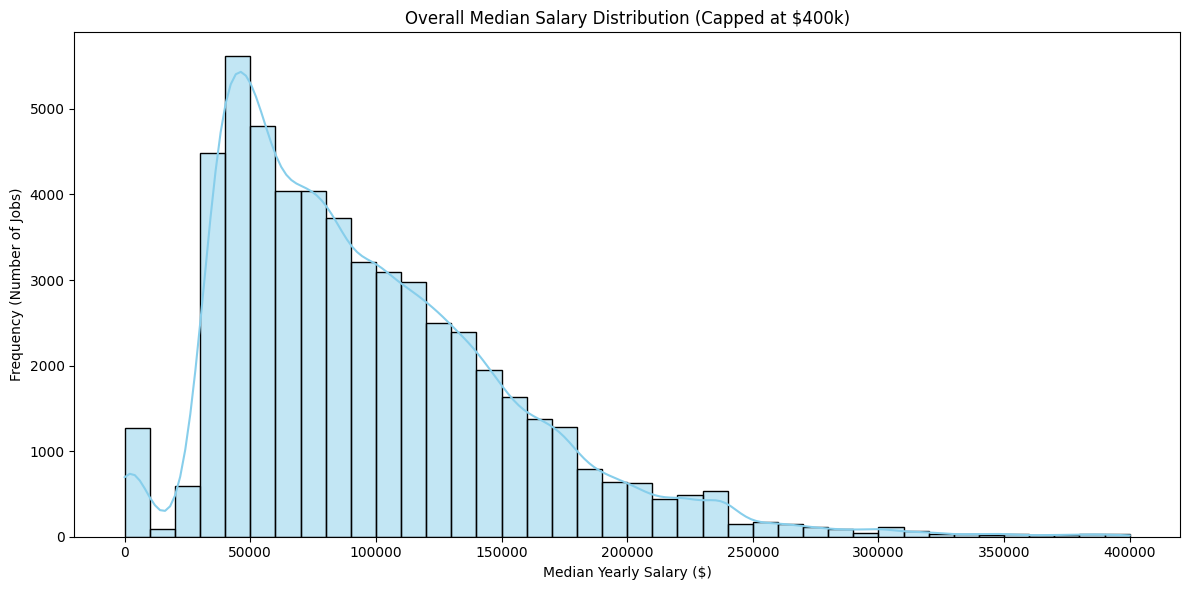
\includegraphics[width=\columnwidth]{output1.png}
    \caption{Median Salary Distribution Histogram}
    \label{fig:salary_dist}
\end{figure}

For exploratory data analysis, we will examine salary distributions overall and across categories such as industry, company size, and location. We will use visualizations including histograms and boxplots to identify patterns and variability in salary data.

To statistically test salary differences across groups, we will conduct hypothesis testing using:

\begin{itemize}
    \item \textbf{ANOVA (Analysis of Variance)} -- a statistical test used to determine whether the average salary differs significantly across multiple groups, such as industries.
    \item \textbf{ANCOVA (Analysis of Covariance)} -- similar to ANOVA, but it controls for additional variables (such as company size or location) to determine whether salary differences remain significant after accounting for those factors.
\end{itemize}

These tests will help us determine whether observed salary differences are statistically meaningful rather than due to random variation.

\section*{5. Approach}

Our approach combines statistical analysis with machine learning techniques.

First, we will preprocess the textual data by cleaning job descriptions and converting them into numerical features using methods such as TF-IDF or word embeddings. This allows the models to interpret text information mathematically.

Next, we will build baseline models using linear regression. Linear regression provides a simple and interpretable starting point for predicting salary based on structured variables (industry, company size, location) and text-based features.

After establishing a baseline, we will experiment with more advanced models such as Support Vector Machines (SVMs) and neural networks. These models can capture more complex and nonlinear relationships between job descriptions and compensation.

By comparing simple and advanced models, we aim to determine whether salary prediction improves significantly when using more flexible modeling techniques.

\begin{figure}[t]
    \centering
    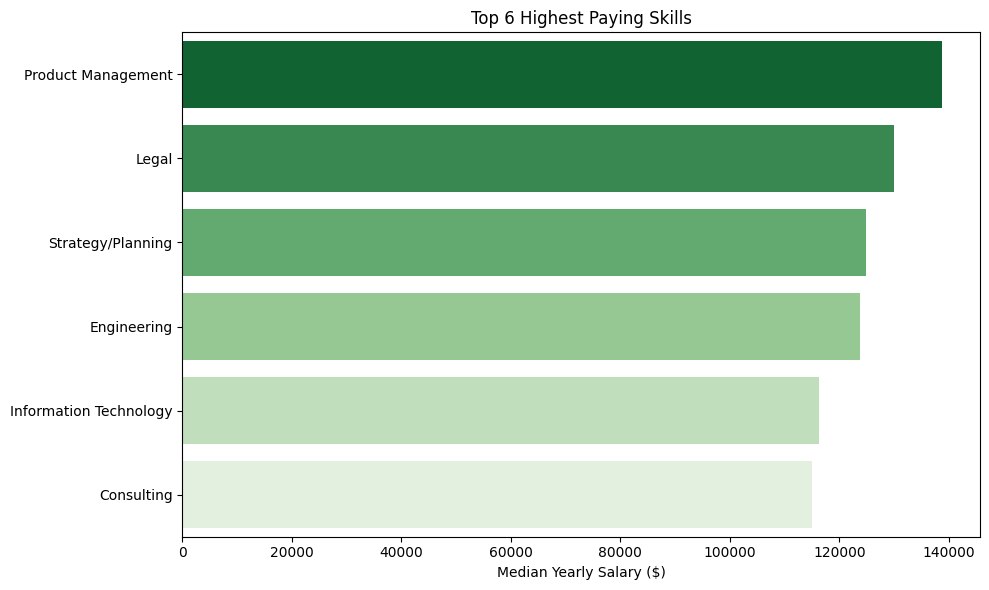
\includegraphics[width=\columnwidth]{output2.png}
    \caption{6 Highest Paying Skills}
    \label{fig:high_paying_skills}
\end{figure}

\begin{figure}
    \centering
    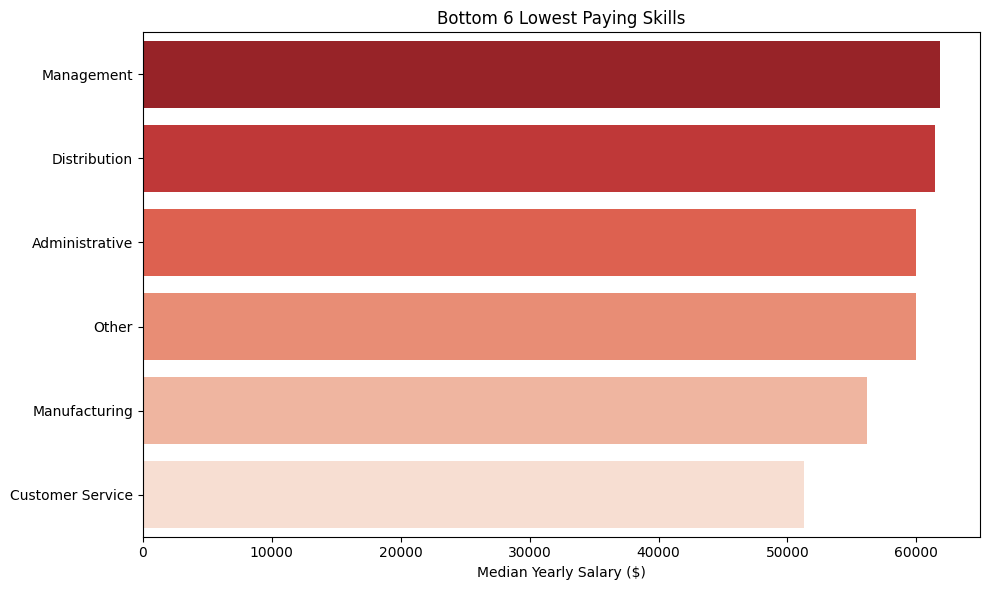
\includegraphics[width=\columnwidth]{output3.png}
    \caption{6 Lowest Paying Skills}
    \label{fig:low_paying_skills}
\end{figure}

\section*{6. Evaluation Metrics}

We will evaluate our results both qualitatively and quantitatively.

Qualitatively, we will produce visualizations such as salary distribution plots, industry comparisons, and the predicted-versus-actual salary scatterplot. These will help us interpret patterns and understand model behavior.

Quantitatively, because salary prediction is a regression problem, we will use:

\begin{itemize}
    \item \textbf{Mean Squared Error (MSE)} -- measures the average squared difference between predicted and actual salaries. Lower values indicate better performance.
    \item \textbf{Root Mean Squared Error (RMSE)} -- similar to MSE but expressed in salary units (dollars), making it easier to interpret the prediction error.
    \item \textbf{R-squared ($R^2$)} -- measures the proportion of salary variation explained by the model. Higher values indicate a stronger explanatory power. 
\end{itemize}

We will also use cross-validation to ensure that our results generalize beyond the training data.

For ANOVA and ANCOVA, we will report p-values and F-statistics to determine whether salary differences between groups are statistically significant.

If advanced models substantially reduce prediction error compared to linear regression, this would suggest that salary depends on complex patterns within job descriptions.

\section*{7. Pre-Processing}
First, we standardize the target variable, \texttt{med\_salary}, by converting all hourly and monthly rates into a consistent yearly figure using conversion factors of $\times 2{,}080$ for hourly rates (40 h/week $\times$ 52 weeks) and $\times 12$ for monthly rates. Where the median salary is missing, we impute it from the mean of the available minimum and maximum bounds. Records with no salary signal whatsoever are dropped.

We then perform a high-integrity merge between \texttt{salaries.csv}, \texttt{postings.csv}, and \texttt{job\_industries.csv} (joined with \texttt{industries.csv}) using \texttt{job\_id} as the primary key. Extreme salary values below \$15{,}000 or above \$600{,}000 per year are removed as implausible outliers, leaving \textbf{35,379 job postings} for modeling. The final merged dataset covers all seven work types, multiple experience levels, and hundreds of industry categories.

For the unstructured text, we normalize job descriptions by stripping HTML tags with a regular expression and removing all non-alphabetic characters. The cleaned text is then lower-cased and reduced to single-space separation, producing a corpus ready for vectorization. Categorical variables (\texttt{work\_type}, \texttt{formatted\_experience\_level}, \texttt{industry\_name}) are label-encoded via one-hot encoding.

\section*{8. Exploratory Data Analysis}
Our exploratory analysis focuses on identifying the primary structural and skill-based drivers of compensation. This phase involved analyzing salary distributions across work types, skill volumes, and specific technical domains to uncover the underlying patterns in the LinkedIn dataset.

\subsection*{Overall Salary Distribution}
As shown in Figure~\ref{fig:salary_dist}, the distribution of annual median salaries is strongly right-skewed with a mode near \$50{,}000--\$60{,}000, consistent with the large proportion of full-time, entry-to-mid-level U.S. positions. A long tail extends toward \$400{,}000, corresponding to executive and specialized technical roles. The presence of this skew motivated our use of a salary cap at \$400{,}000 in exploratory plots and a broader \$600{,}000 ceiling for modeling (to include senior executive postings while discarding clearly erroneous data entry). The salary distribution also highlights that approximately 8\% of postings fall below \$20{,}000, a cluster that largely represents part-time and internship roles already distinguished by \texttt{work\_type}.

\subsection*{a. Work Type Spread}
Shown in Figure~\ref{fig:work_type}, there is significant variance in salary across different employment categories. Full-time and Contract roles exhibit the highest median salaries and the widest ranges, with several postings reaching the \$400,000 cap. In contrast, Internship, Part-time, and Volunteer roles cluster at the lower end of the spectrum, usually below \$75,000, suggesting that \texttt{work\_type} is a critical categorical feature for our regression models.

\begin{figure} [h]
    \centering
    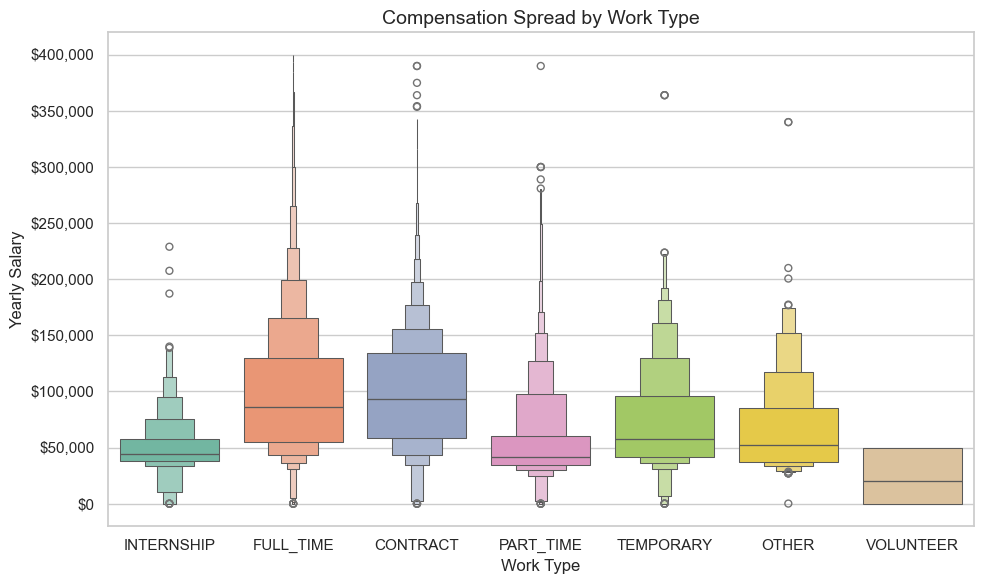
\includegraphics[width=\columnwidth]{output4.png}
    \caption{Compensation Spread by Work Type}
    \label{fig:work_type}
\end{figure}

\subsection*{b. Skill Requirement Volume}
Since our dataset contains jobs that listed multiple skills, we plotted the median salary for jobs listing multiple unique skills. Interestingly, we see that requiring 2 unique skills averages a lower median salary than having 1 and 3. This "threshold effect" suggests that jobs requiring a specific trifecta of skills are valued significantly higher by employers, justifying our plan to use non-linear models like Neural Networks to capture these complex interactions.

\begin{figure}[h]
    \centering
    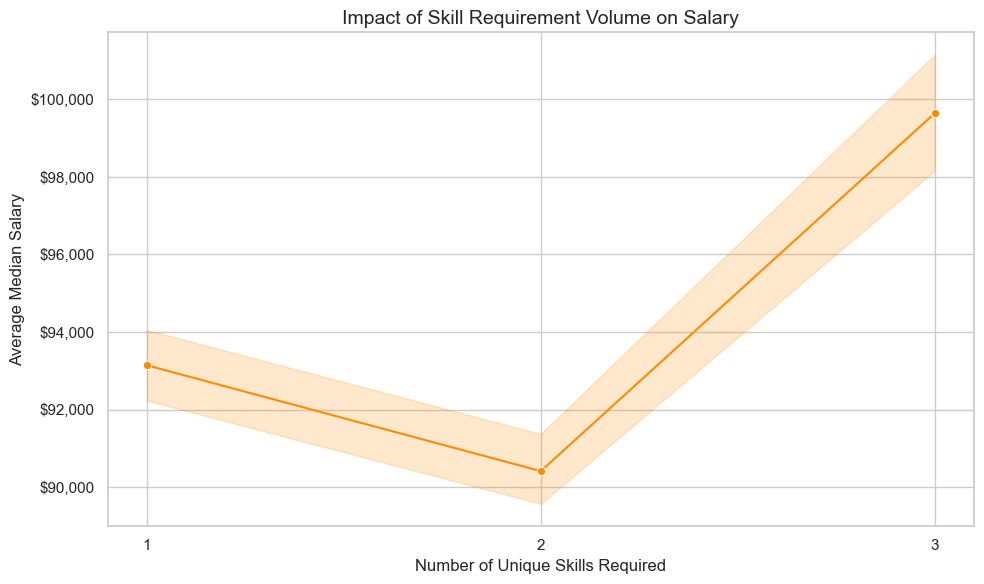
\includegraphics[width=\columnwidth]{output5.png}
    \caption{Impact of Skill Requirement Volume on Salary}
    \label{fig:skill_volume}
\end{figure}

\subsection*{c. Salary Distribution for Demanded Skills}
We gathered the 5 most frequent industry categories from the dataset and graphed a box plot. We see that Engineering and Information Technology contains the highest median salary listing at above \$100,000. In contrast, Management and Sales roles show lower median pay and narrower interquartile ranges. Manufacturing roles exhibit the lowest median pay among the top five.

\begin{figure}[h]
    \centering
    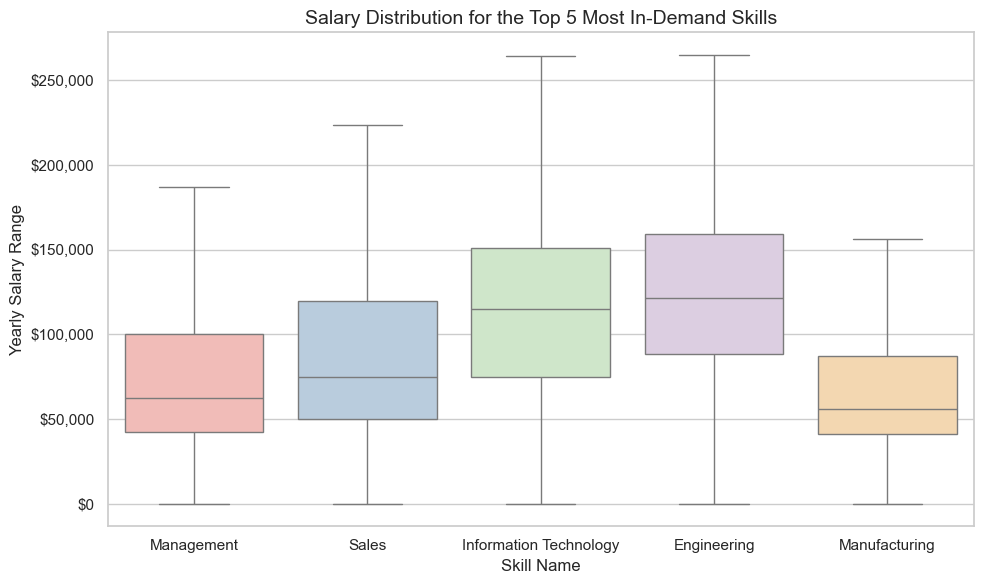
\includegraphics[width=\columnwidth]{output6.png}
    \caption{Salary Distribution for Most In-Demand Skills}
    \label{fig:industry_dist}
\end{figure}

\subsection*{d. Key Observations from EDA}
Several structural patterns emerged that directly informed our modeling decisions. First, \texttt{work\_type} is the single strongest categorical predictor: full-time and contract roles command median salaries roughly 2$\times$ higher than internships and part-time roles. Second, the non-monotonic relationship between skill count and salary (Figure~\ref{fig:skill_volume}) suggests interaction effects that linear models may struggle to capture, motivating the use of non-linear models in future work. Third, the high-paying skills bar chart (output2) shows that niche technical qualifications such as quantum computing and chip architecture carry strong premiums, while low-paying postings (output3) tend to emphasize generic soft skills. This asymmetry validates the use of TF-IDF text features: salary signal is concentrated in specific vocabulary rather than general language patterns.

\section*{9. Statistical Analysis}
To validate our hypotheses, we conducted two primary statistical tests:

\subsection*{a. One-Way ANOVA}
We tested if salary median changes significantly based on required skills. We performed a One-Way ANOVA test on skills for job listings.

\textbf{Results:}The test resulted in an F-statistic of 4.3275 and a p-value of 0.001685. The extremely small p-value indicates that the differences in salary across these skill categories are statistically significant, justifying their use as key features in our predictive models.

\subsection*{b. Two-Sample T-Test}
We conducted a t-test to compare the average salaries of roles requiring specific high-value skills (e.g., Information Technology) against the general population.

\textbf{Results:}The test yielded a p-value of 0.0144. Since the p-value is below the $0.05$ threshold, we reject the null hypothesis and conclude that the targeted skill significantly influences salary levels.



\section*{10. Model Training and Evaluation}

\subsection*{a. Feature Representation}

We built two versions of the model to see whether job description text improves salary prediction:

\begin{itemize}
    \item \textbf{Model A (structured only):} Uses categorical job information -- work type, experience level, and industry -- converted into numerical format.
    \item \textbf{Model B (structured + text):} Everything in Model A, plus text features from job descriptions. We used TF-IDF, which turns words into numbers based on how often they appear and how unique they are. We kept the top 5{,}000 words/phrases to capture the most useful vocabulary.
\end{itemize}

\subsection*{b. Model}

Both models use Ridge Regression, a form of linear regression that adds a penalty to prevent the model from over-relying on any single word or feature -- especially important when dealing with thousands of text features. We split the data 80/20: 28{,}303 jobs for training and 7{,}076 for testing.

\subsection*{c. Results}

Table~1 shows how well each model predicted salary on the test set.

\begin{table}[h]
\centering
\resizebox{\columnwidth}{!}{%
\begin{tabular}{lcc}
\hline
\textbf{Model} & \textbf{RMSE (\$)} & \textbf{$R^2$} \\
\hline
Model A: Structured only         & 47{,}754 & 0.320 \\
Model B: Structured + TF-IDF     & 36{,}843 & 0.595 \\
\hline
\multicolumn{3}{l}{\textit{5-Fold CV (Model B): $R^2 = 0.594 \pm 0.015$,}} \\
\multicolumn{3}{l}{\textit{\phantom{5-Fold CV (Model B): }RMSE $= \$36{,}998 \pm \$1{,}432$}} \\
\hline
\end{tabular}%
}
\caption{Test-set performance of Ridge Regression models.}
\label{tab:model_results}
\end{table}

Adding text features cut prediction error by \textbf{\$10{,}911} (23\%) and raised $R^2$ from 0.320 to 0.595, meaning the model now explains roughly 60\% of salary variation. Cross-validation scores closely matched these results, showing the model generalizes well to unseen data.

\begin{figure}[h]
    \centering
    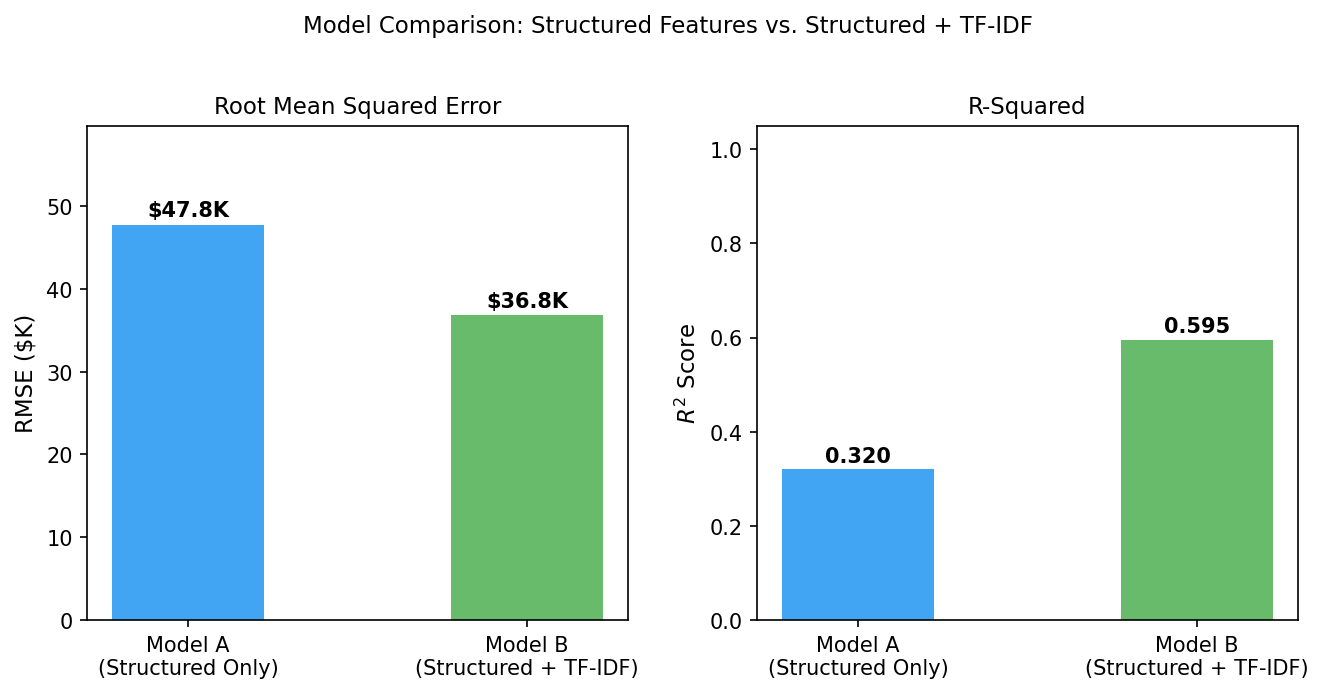
\includegraphics[width=\columnwidth]{output10.png}
    \caption{Model comparison: RMSE and $R^2$ for Model A vs.\ Model B.}
    \label{fig:model_comparison}
\end{figure}

\begin{figure}[h]
    \centering
    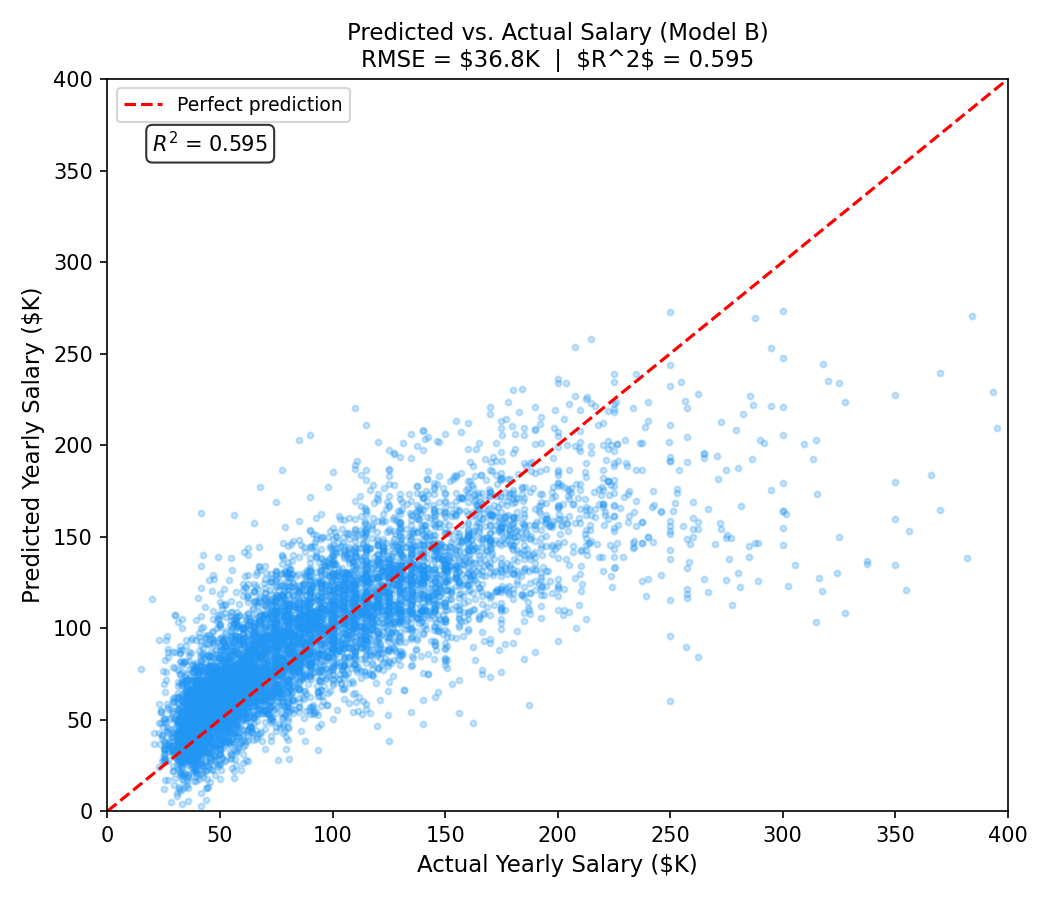
\includegraphics[width=\columnwidth]{output7.png}
    \caption{Predicted vs.\ actual salary on the test set (Model B). The dashed red line represents perfect prediction.}
    \label{fig:pred_vs_actual}
\end{figure}

\begin{figure}[h]
    \centering
    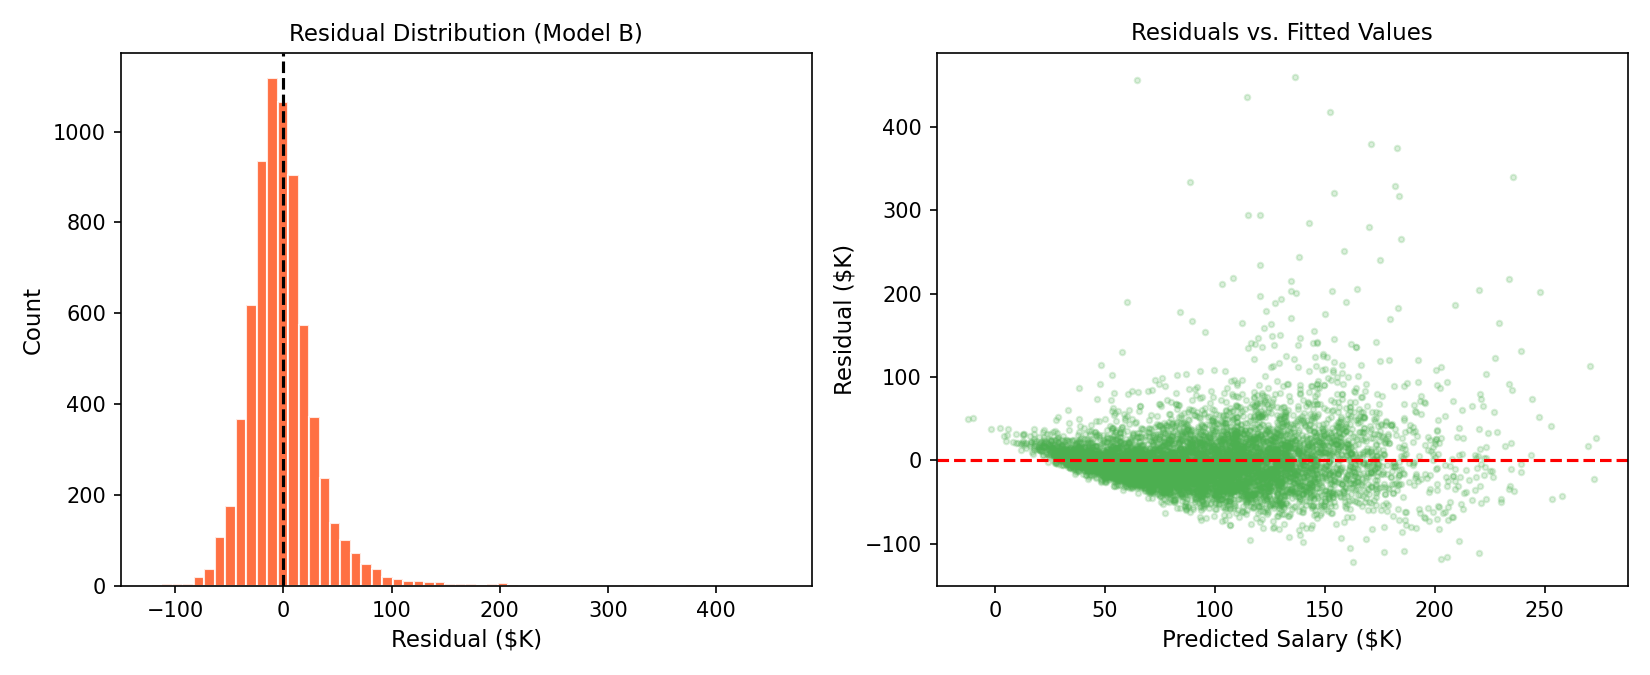
\includegraphics[width=\columnwidth]{output8.png}
    \caption{Residual distribution and residuals vs.\ fitted values for Model B.}
    \label{fig:residuals}
\end{figure}

\begin{figure}[h]
    \centering
    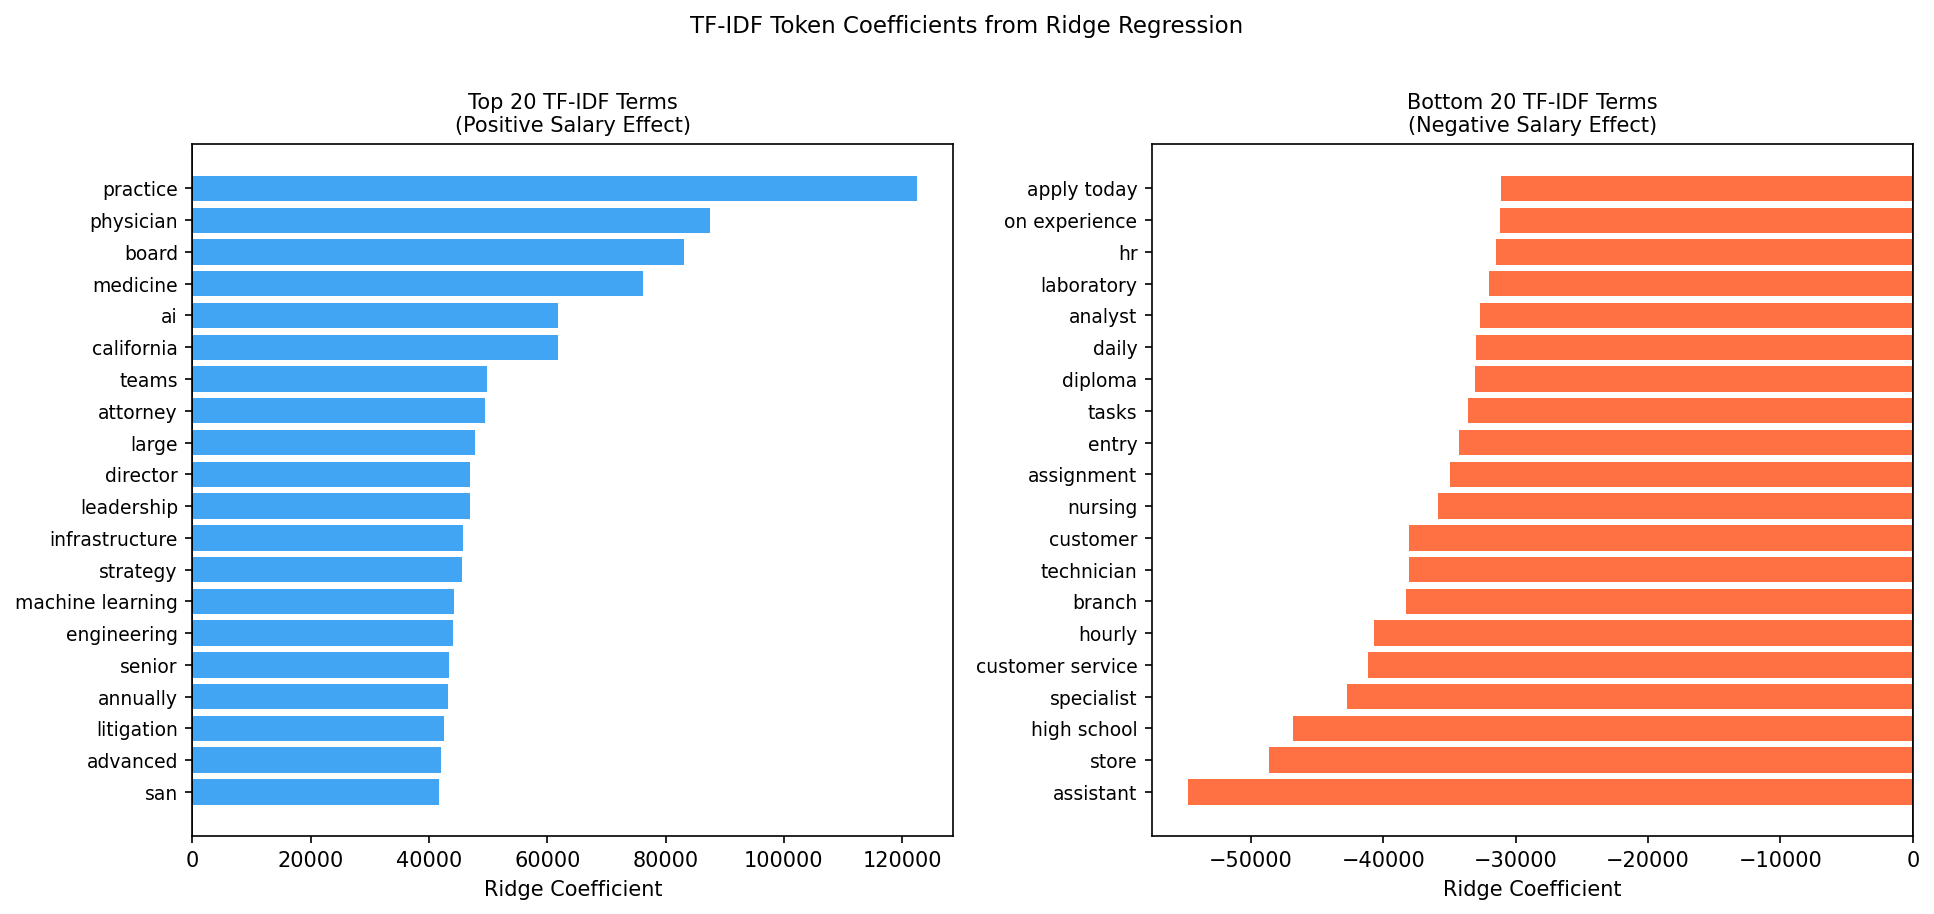
\includegraphics[width=\columnwidth]{output9.png}
    \caption{Top 20 TF-IDF tokens with the largest positive (left) and negative (right) Ridge coefficients.}
    \label{fig:tfidf_coefs}
\end{figure}

\subsection*{d. What the Words Tell Us}

Figure~\ref{fig:tfidf_coefs} shows which words in job descriptions are most associated with higher or lower salaries. Words linked to high pay tend to be technical terms from fields like machine learning, finance, and cloud computing. Words linked to lower pay tend to come from service-sector jobs (e.g., shift scheduling, customer service). This aligns with our EDA findings and confirms that salary information is encoded in specific vocabulary, not just general language.

\subsection*{e. Residual Analysis}

The residual plot (Figure~\ref{fig:residuals}) shows how far off our predictions were. Errors are roughly centered at zero, but the model tends to under-predict the highest salaries -- a common issue with linear models when salaries are heavily skewed. Prediction error also grows at higher salary levels, suggesting that future work with non-linear models or a log-transformed salary target could improve accuracy for senior roles.

\subsection*{f. Challenges}

\begin{itemize}
    \item \textbf{Limited salary data.} Only 35,379 of 120,000+ postings had usable salary info after cleaning -- a 71\% reduction -- limiting how broadly our model applies.
    \item \textbf{Many features, limited data.} With 5{,}000 text features and \textasciitilde28k samples, regularization was essential to prevent overfitting.
    \item \textbf{Growing prediction error.} The model struggles more with high-salary roles; future work will explore log-transformation or non-linear models.
    \item \textbf{Missing experience levels.} About 30\% of postings had no experience level listed and were labeled ``Unknown,'' which may weaken that feature's usefulness.
    \item \textbf{Too many industry categories.} Hundreds of fine-grained industries means rare ones have very few examples. Grouping small industries into an ``Other'' category may help in future iterations.
\end{itemize}

\section*{11. Neural Network Model}

\subsection*{a. Motivation}

The residual analysis from our Ridge Regression models revealed a consistent pattern: prediction error grew at higher salary levels, and the model struggled to capture non-linear relationships in the data. Our EDA also showed a non-monotonic relationship between skill count and salary, which a linear model cannot easily represent. To address these limitations, we trained a Multilayer Perceptron (MLP) neural network as our advanced model. An MLP can learn complex, non-linear patterns by passing data through multiple layers of interconnected nodes, each applying a transformation before passing the result forward.

\subsection*{b. Dataset and Features}

To keep training time manageable on CPU, we worked with a random sample of 10{,}000 postings drawn from the full 35{,}379-posting dataset, using the same random seed as the Ridge experiments for reproducibility. The sample was split 80/20 into 8{,}000 training and 2{,}000 test examples. We used the same two feature configurations as in Section~10, yielding four models in total for comparison.

\begin{itemize}
    \item \textbf{Model C (MLP, structured only):} Work type, experience level, and industry, one-hot encoded and normalized with a standard scaler.
    \item \textbf{Model D (MLP, structured and TF-IDF):} All structured features from Model C plus TF-IDF text vectors from job descriptions, scaled with a max-absolute scaler to preserve the sparse structure of the text features.
\end{itemize}

\subsection*{c. Architecture and Training}

Both neural network models use a four-layer architecture with hidden layer sizes of 512, 256, 128, and 64 neurons respectively. Each layer uses a ReLU activation function, which simply sets any negative value to zero and passes positive values through unchanged. This allows the network to learn non-linear salary patterns without the vanishing-gradient problems that come with older activation functions.

We trained using the Adam optimizer with an initial learning rate of 0.001 and L2 regularization (weight decay) of 0.01 to prevent overfitting. Batch size was set to 256 samples per update. To avoid over-training, we enabled early stopping: training halts automatically when the validation score does not improve by more than 0.0001 for 10 consecutive epochs. The validation set was 10\% of the training data held aside during training.

\subsection*{d. Results}

Table~2 shows the test-set performance for all four models across both algorithms.

\begin{table}[h]
\centering
\resizebox{\columnwidth}{!}{%
\begin{tabular}{llcc}
\hline
\textbf{Model} & \textbf{Algorithm} & \textbf{RMSE (\$)} & \textbf{$R^2$} \\
\hline
Model A & Ridge, structured only        & 46{,}748 & 0.290 \\
Model B & Ridge, structured + TF-IDF    & 37{,}190 & 0.551 \\
Model C & MLP, structured only          & 46{,}657 & 0.293 \\
Model D & MLP, structured + TF-IDF      & \textbf{36{,}947} & \textbf{0.557} \\
\hline
\end{tabular}%
}
\caption{Test-set performance across all four models (10{,}000 sample).}
\label{tab:nn_results}
\end{table}

Model D achieved the best performance overall, with an RMSE of \$36{,}947 and an $R^2$ of 0.557. It reached this result in just 27 epochs before early stopping triggered. Adding TF-IDF text features again provided the largest single improvement across both algorithms, reducing RMSE by roughly \$10{,}000 compared to structured features alone. The full four-model comparison is visualized in Figure~\ref{fig:nn_comparison}.

\begin{figure}[h]
    \centering
    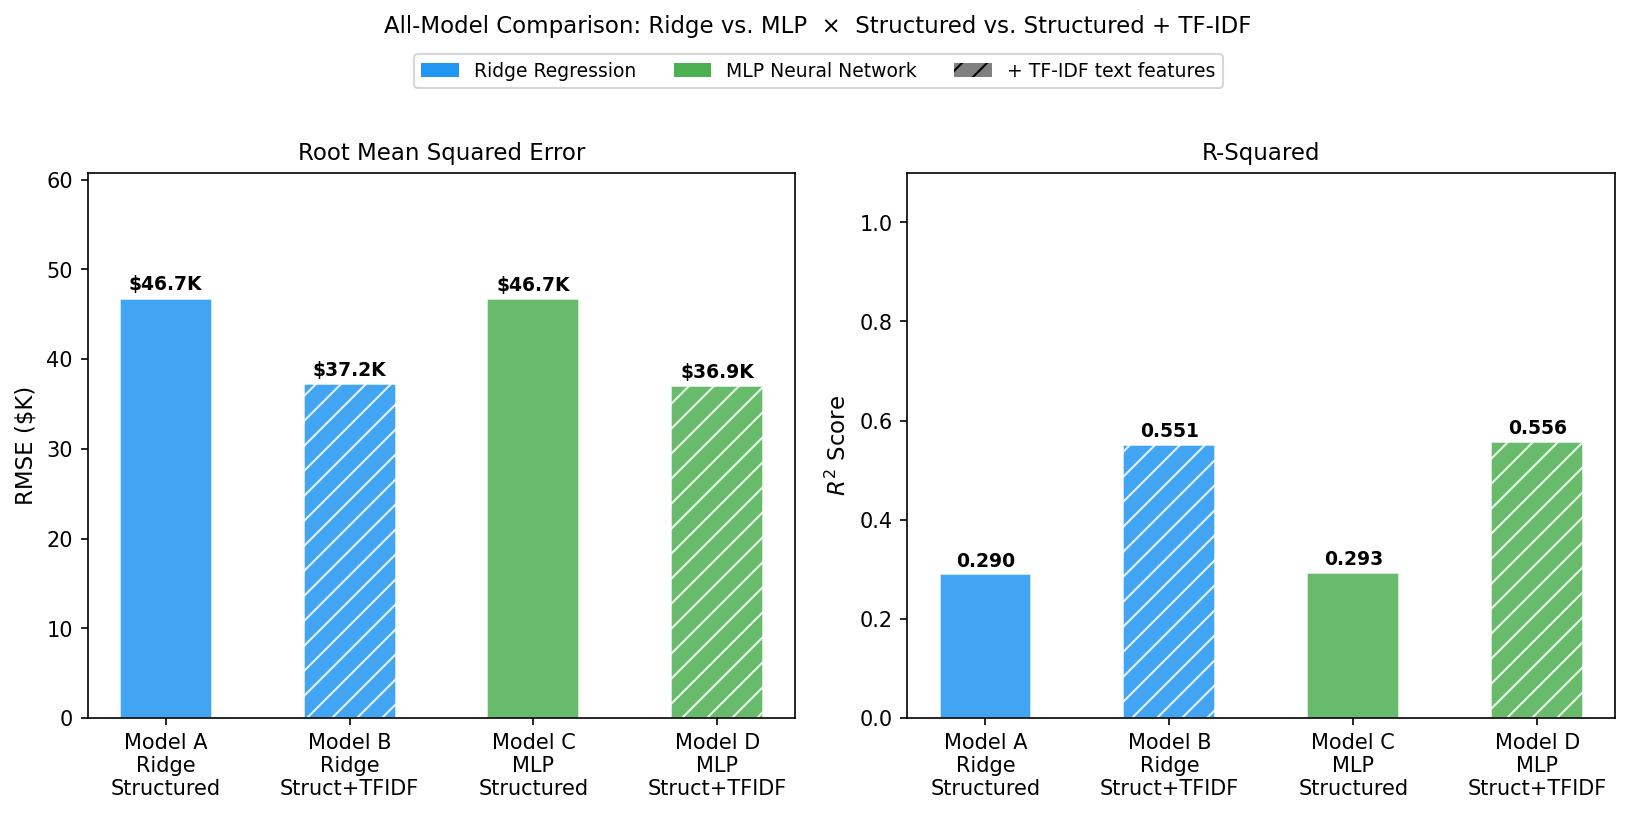
\includegraphics[width=\columnwidth]{nn_output4.png}
    \caption{RMSE and $R^2$ comparison across all four models. Blue bars represent Ridge Regression and green bars represent the MLP. Hatching indicates that TF-IDF text features were included.}
    \label{fig:nn_comparison}
\end{figure}

\begin{figure}[h]
    \centering
    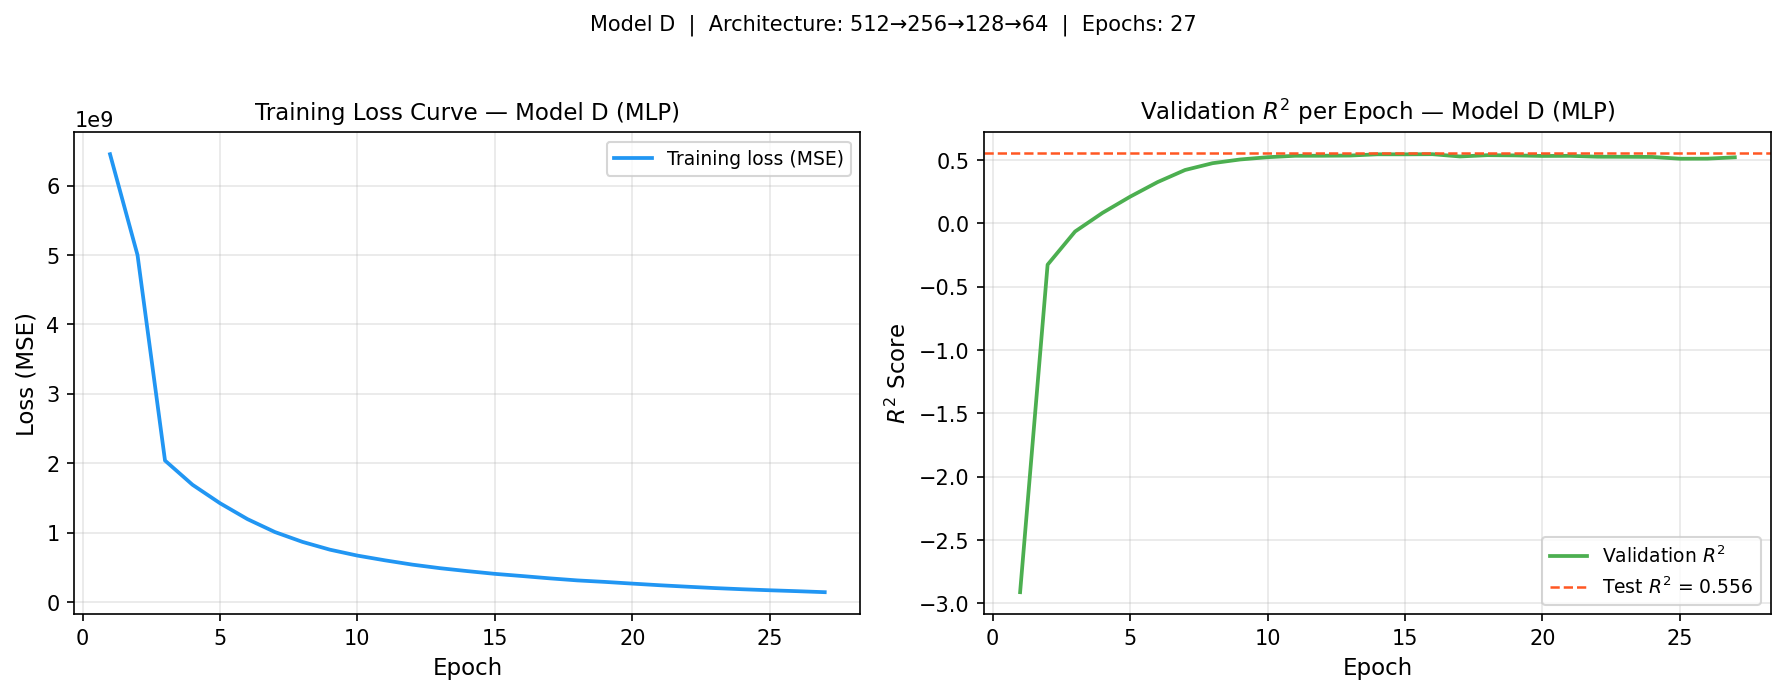
\includegraphics[width=\columnwidth]{nn_output1.png}
    \caption{Training loss and validation $R^2$ per epoch for Model D. The model converged in 27 epochs before early stopping halted training.}
    \label{fig:nn_loss}
\end{figure}

\begin{figure}[h]
    \centering
    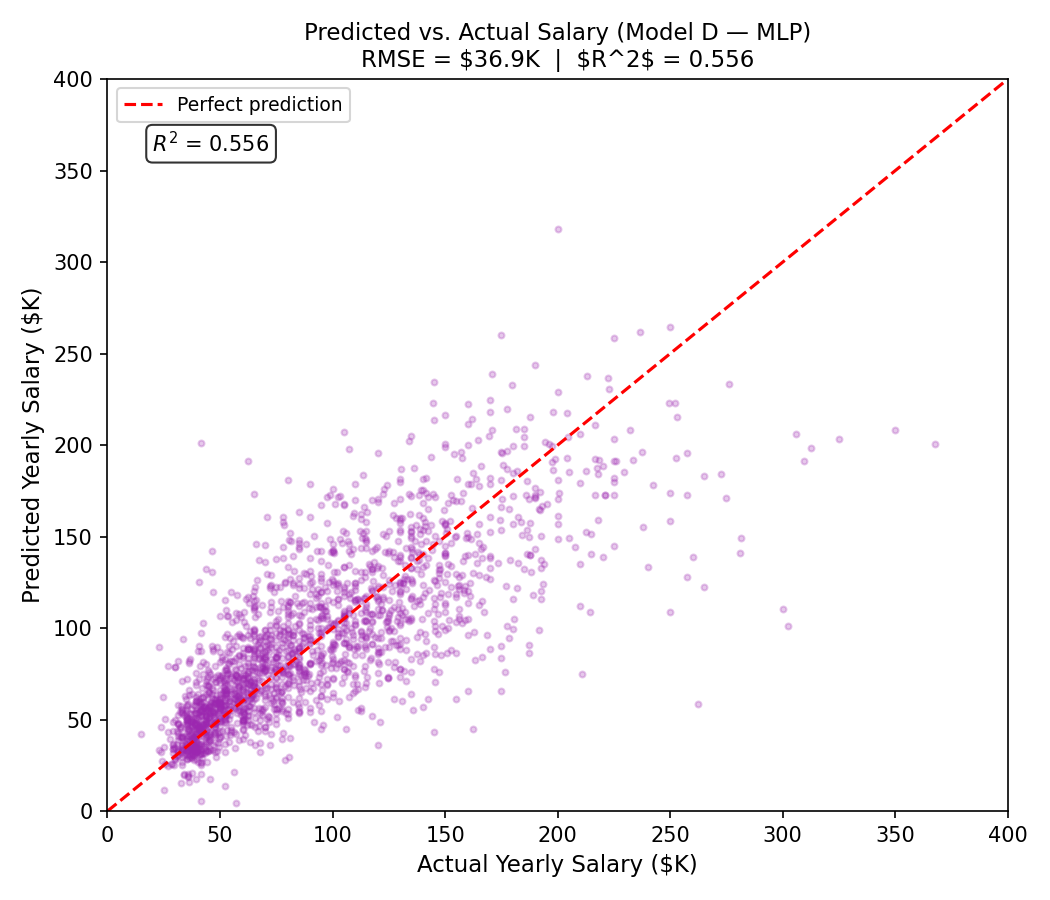
\includegraphics[width=\columnwidth]{nn_output2.png}
    \caption{Predicted vs.\ actual salary on the test set for Model D. The dashed red line represents perfect prediction.}
    \label{fig:nn_pred}
\end{figure}

\begin{figure}[h]
    \centering
    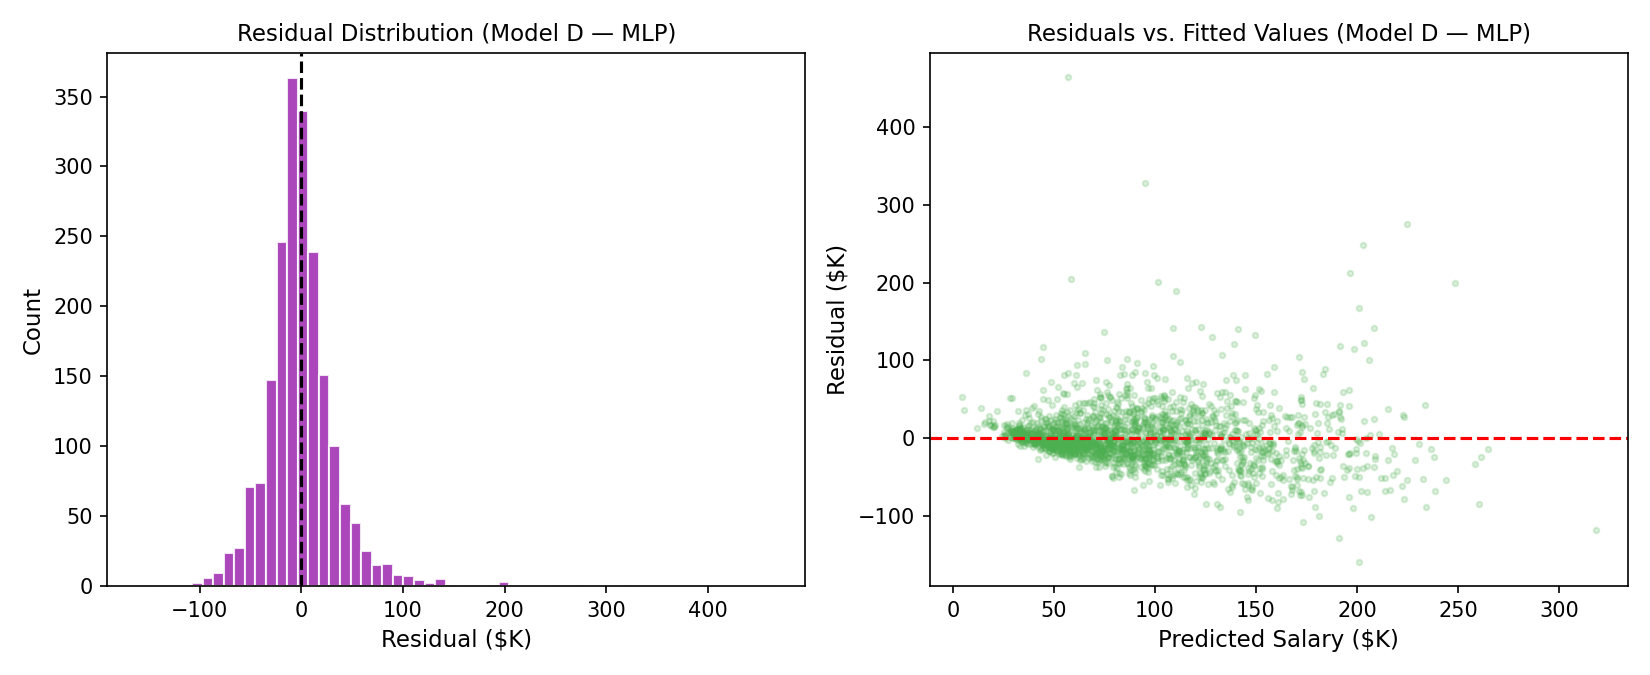
\includegraphics[width=\columnwidth]{nn_output3.png}
    \caption{Residual distribution and residuals vs.\ fitted values for Model D.}
    \label{fig:nn_resid}
\end{figure}

\subsection*{e. Training Curve}

Figure~\ref{fig:nn_loss} shows how the model improved over training epochs. The training loss dropped sharply in the first few epochs, falling from over 6 billion to under 500 million in the first 12 iterations. The validation $R^2$ climbed quickly at first, reaching around 0.53 by epoch 12, after which improvement slowed and the model stopped at epoch 27. This pattern is healthy: rapid early learning followed by a gradual plateau, with no sign of catastrophic overfitting.

\subsection*{f. Comparison with Ridge Regression}

The MLP outperformed Ridge Regression on both RMSE and $R^2$ when text features were included, but the margin was narrow. Model D (MLP) achieved an $R^2$ of 0.557 compared to 0.551 for Model B (Ridge), a modest 0.6 percentage point improvement. On structured features alone, the two algorithms performed almost identically, with Model C edging out Model A by less than \$100 in RMSE.

This result suggests two things. First, the salary signal in this dataset is largely captured by linear relationships between features and compensation. The MLP did not find dramatically different patterns from those Ridge already exploited. Second, the text vocabulary encoded through TF-IDF is the dominant source of predictive information regardless of which algorithm is used. The word choice in a job description matters far more than which model reads it.

\subsection*{g. Residual Analysis}

The residual plots for Model D (Figure~\ref{fig:nn_resid}) closely resemble those of Model B. Errors are roughly centered at zero with a slight positive skew, meaning the MLP also tends to under-predict the highest salaries. The fan-shaped spread in the residuals-vs.-fitted plot indicates that prediction error grows with salary level, a pattern consistent with the skewed salary distribution in the raw data. This heteroscedasticity suggests that future work using a log-transformed salary target or a more expressive architecture could further reduce error at the high end of the pay scale.

\subsection*{h. Challenges}

Training the MLP on this dataset surfaced a few practical difficulties. Converting the sparse TF-IDF matrix to a dense array for the neural network required roughly 500 MB of memory, which slowed down processing on a standard laptop CPU. Training each epoch on the full dataset took approximately two minutes, making cross-validation impractical without access to a GPU or a computing cluster. We addressed this by subsampling to 10{,}000 rows, which reduced training time to under ten minutes while preserving the core patterns in the data. The slight drop in absolute performance compared to Section~10 (where Ridge was trained on all 35{,}379 rows) reflects this trade-off between speed and dataset coverage rather than any fundamental weakness of the neural network architecture.


\section*{12. Future Work}

Several directions could improve upon our results. First, applying a logarithmic transformation to \texttt{med\_salary} would address the heteroskedasticity observed in both models, likely reducing error for high-salary roles. Second, replacing TF-IDF with contextual embeddings from a pre-trained model such as BERT could capture phrase-level semantics that bag-of-words representations miss. Third, training the MLP on the full 35{,}379-posting dataset with GPU acceleration would provide a fairer comparison against the Ridge baseline. Finally, imputing missing experience levels from job description text and consolidating rare industry categories into broader groups could strengthen the structured features.

\section*{13. Conclusion}

This project demonstrated that job description text is the dominant predictor of salary in LinkedIn job postings. Across both Ridge Regression and MLP models, adding TF-IDF features reduced RMSE by roughly \$10{,}000 and raised $R^2$ from approximately 0.29 to 0.56 --- a larger gain than switching algorithms entirely. Statistical tests confirmed that skill category significantly influences compensation ($F = 4.33$, $p = 0.0017$). The primary limitation is heteroscedasticity: both models under-predict high salaries, pointing toward log-transformed targets and richer text representations as the most promising directions for future work. Overall, our results confirm that the market value of professional skills is recoverable from publicly available job posting data.


\bibliography{refs}

\end{document}
